\documentclass[conference]{IEEEtran}

%+++++++++++++++++++++++++++++++++++++++++++++++++++
\usepackage[pdftex]{graphicx}
\usepackage{amsmath}
\usepackage{eqparbox}
%+++++++++++++++++++++++++++++++++++++++++++++++++++

\hyphenation{op-tical net-works semi-conduc-tor IEEEtran}
\begin{document}

%+++++++++++++++++++++++++++++++++++++++++++++++++++++++++++++++++++++++++++++++++++++++++
\title{\LARGE SUNFLOWER: A Trust Execution Environment on RISC-V \\Based on Tagged Memory}
\author{\authorblockN{Xu Jinyan 3160101126 Duan Yuxuan 3160105210 Lin Yizhu 3160104229} }
%+++++++++++++++++++++++++++++++++++++++++++++++++++++++++++++++++++++++++++++++++++++++++

\maketitle
\setlength{\parskip}{0.4\baselineskip}


% ================
% # Abstract     #
% ================

\begin{abstract}
This is a report for the class: Network Security Theory and Practice, our project is aimed to build a execution environment in RISC-V using tagged memory technology. RISC-V is an open and extensible instruction set architecture designed by UC Berkly, because of its low overhead, it's very suitable for using in the embedded devices and Internet of things. As with the various system vulnerabilities recently exposed, operating systems are no longer fully trusted. More and more people choose to using the hardware security method, like Trust Zone(ARM), SGX(Intel). However, there are still no officially supported safety standards for RISC-V.

Here, we design a tagged memory hardware security architecture, inspired by the paper[1]. Tagged memory has been proposed as a fine-grained security mechanism to support protection of data flow, pointers or capabilities for a long time, but none of the existing schemes provide efficient and flexible at the same time, it is still a open problem. We using tag-aware instruction and a simple kernel to achieve a fine-grained isolation. We also provide a series of tools for easy to use, a gcc and objdump supported tag-aware instructions. And we finish our logical design in Spike, a RISC-V simulator.
\end{abstract}

\begin{keywords}
RISC-V, tagged memory, tag-aware instruction set architecture.\\
\end{keywords}


% ========================
% # I. Introduction      #
% ========================

\section{Introduction}
IoT devices are rapidly entering everyday life. However, these devices have a great risk to be attacked since the code of these devices are complex thus potential to have bugs. To ensure the security of the applications running on these devices even when the devices are compromised, a kind of skill called Trusted Execution Environment(TEE) can be of great help. The main idea of TEE is to use isolated execution to protect trusted applications from compromised operating systems or other untrusted software on the same device.

Recent years have witnessed many implementations of TEE on different systems. ARM TrustZone and Intel SGX are two widely applied TEE architectures. ARM TrustZone divides the computer resources into a secure and non-secure world on hardware level.\cite{TrustZone} The secure world can access all system resources while the non-secure world can only access data in the non-secure world or call secure applications through designed secure entry points. With TrustZone architecture, if sensitive data and code are hidden in the secure world, they cannot be accessed by untrusted applications or system. However, TrustZone needs a secure kernel to manage the secure world, providing secure system services, thus enlarge the trusted computing base(TCB), which increases the risk. Intel SGX uses an isolated container called enclave which hold sensitive part of applications.\cite{SGX} Unlike TrustZone, SGX does not need any privileged supervisor like a trusted kernel, thus reduces TCB. But SGX needs complex instructions to manage enclaves.

Resource-constrained devices like IoT devices often have little memory, thus needs fine-grained memory management. The isolation boundary the existing implementations of TEE provides are not fine-grained enough for small IoT devices to apply. Inspired by the work in \cite{TIMBERV}, we use a technique called \emph{tagged memory} to provide flexible isolation for low-end devices. The main method of tagged memory technique is to associate memory blocks with additional metadata called tag, used for access control and other memory management. There have been active new research on tagged memory, such as use this technique help data flow tracking.\cite{HDFI}. However current tagged memory scheme are not efficient enough on small IoT devices\cite{TIMBERV}, which is the aim of our work.

This work is based on the instruction set architecture RISC-V.\cite{RISCV} RISC-V is suitable for development on IoT devices due to its simple instruction architecture. Also it is open and support instruction extension. On the other hand, the scheme which uses tagged memory technique to implement TEE hasn't been supported on RISC-V. These are the reasons why we choose to implement our work on RISC-V. RISC-V defines three different privilege mode: machine-mode(M), supervisor-mode(S) and user-mode(U). M-mode can access all the system resources and are meant for emulating the machine, while S-mode and U-mode are respectively used by operate systems and user applications.

In this work, we present SUNFLOWER, a RISC-V based TEE implementation with tagged memory applied. This is a hardware-software co-design work. In the hardware level, we add instructions that can load and store data with tag check to the RISC-V simulator spike. In the software level, we provide a secure interface for applications to call and set part of their code or data with trusted tag. We associate each memory word with 2 bits tag, thus achieve fine-grained isolation with low overhead. We estimate our work on a simple encryption program and prove it can work as expected. 

This report will introduce our design frame and details of hardware and software design, followed by evaluation and analysis of our work.


% ====================
% # II. Design Frame #
% ====================

\section{SUNFLOWER Design Frame}
This work is a hardware and software co-design. The hardware design is based on a RISC-V simulator called spike, while the software part is designed on Amazon FreeRTOS embedded system. To support the tagged memory in our work, a tag-aware instruction set is designed as an extension to the original RV64 ISA of RISC-V. This instruction set includes instructions to visit memory unit with tags, helping our system realize access control to memory with different tags. The instruction decoder and MMU are also modified according to the structure of this newly designed instruction set. On the system layer, we design and implement a set of system services, which are run in high privilege mode and perform services like tag update.


% ==========================
% # III. Design Details #
% ==========================

\section{Design Details}
In this section, we will introduce our hardware-software co-design system in detail. In general hardware design includes the implementation of different tags and tag-aware instruction sets, as well as the modification on the datapath and decoder of CPU, while the software part is more close to encapsulate these operating system calls and memory management. 

\subsection{Hardware Design}
To implement tagged memory aided trusted execution environment, the most basic part is to modify the hardware so that it can support tagged memory. We design a 2-bit tag system and a tag-aware instruction set to visit memory with tags, as shown in figure \ref{fig:memory}. In order to satisfy new instructions, which we need to do load and store with tag check, we extend the original CPU and other hardware basis to support them. 

\begin{figure}
	\centering{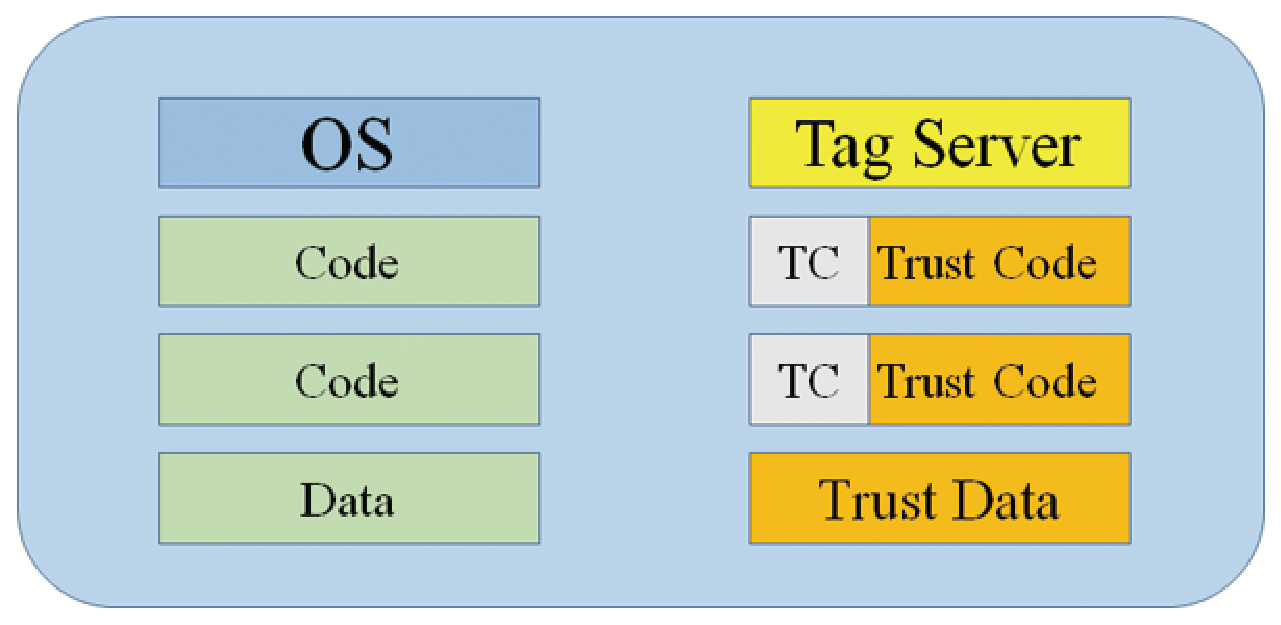
\includegraphics[width=0.9\columnwidth]{asset/memory.eps}}
	\caption{To implement tagged memory aided trusted execution environment, the most basic part is to modify the hardware so that it can support tagged memory. We design a 2-bit tag system and a tag-aware instruction set to visit memory with tags.}
	\label{fig:memory}
\end{figure}

\subsubsection{Tag System Design}
Memory tags in SUNFLOWER system each has 2 bits, resulting in 4 different types of tags, which are N-tag, TU-tag, TS-tag and TC-tag, respectively representing normal mode, trusted user mode, trusted supervisor mode and trusted entry. To be more specific, N-tag is for memory in normal world(not trusted), namely the opposite side of secure world(trusted); TU-tag is for code, namely text, and data in user-mode trusted enclaves, while TS-tag is in supervisor-mode trusted enclaves. TC-tag is for entry point from normal state to trusted state. The design of TC-tag is not redundant since we are supposed to mark where the trusted text begins and defense that kind of attack, which jumps into enclave from other unsafe places. It is designed just for instructions, not for data, which is different from the others. And for data, we use TU-tag to mark it belongs to secure world and TC-tag in the beginning is not needed.

\subsubsection{Tag-aware Instructions}
We extend the original RISC-V instruction architecture with a set of tag-aware instructions to support tagged memory operations. The newly designed instructions are based on I/S type instructions and can perform access control for load and store operations according to the destination memory tag, shown in Figure \ref{fig:LSCT}. Basically, we just view these as a profession version of load and store instruction, which could check and restore memory tag. In addition, the architecture has different granularities of these instructions, such as byte, word and double word, and unsigned counterpart.

The original load instructions are extended to be load check tag instructions(LCT). LCT instructions can compare the tag of the destination memory unit with the expected tag specified in the instruction, check if this load request is legal, and raise exception if it abuses the tag isolation policy. The high 12 bits of the original I-type instructions is immediate operator, used as address offset. We use the highest 2 bits to store the expected tag, denoted as etag. For different granularities, there are lbct, lhct, lwct, ldct for signed size and lbuct, lhuct, lwuct for unsigned ones.

Similarly, the original store instructions are extended to be store check tag instructions(SCT). SCT instructions work the same as LCT instructions, store to destination memory unit if the memory tag and the expected tag match and raise exception if they don't. Besides store instructions also need another 2-bit tag for replacing current memory's tag, denoted as ntag. The immediate fields in S-type instructions consists of the high 7 bits and 8-12 4 bits, used for offset in addressing. The highest 2 bits are used to store tags. The same as LCT, there are sbct, shct, swct and sdct, but not unsigned type.

This design that takes 2 bits from the original immediate fields will affect the addressing space size. The original addressing space is from -4096 to 4096. Hence we use script to transform indirect addressing with a much closer base address. For example, we could not reach 4096 by just using check instructions. But we could replace it with adding its base address with 4096 then set offset 0. From another angle, the range is much wider.

Above checked load or store instructions are defined through RISC-V port. Luckily, RISC-V allows users to make custom instructions and leave four empty slots to insert. And our checked instructions occupies custom 0 and 1.

\begin{figure}
	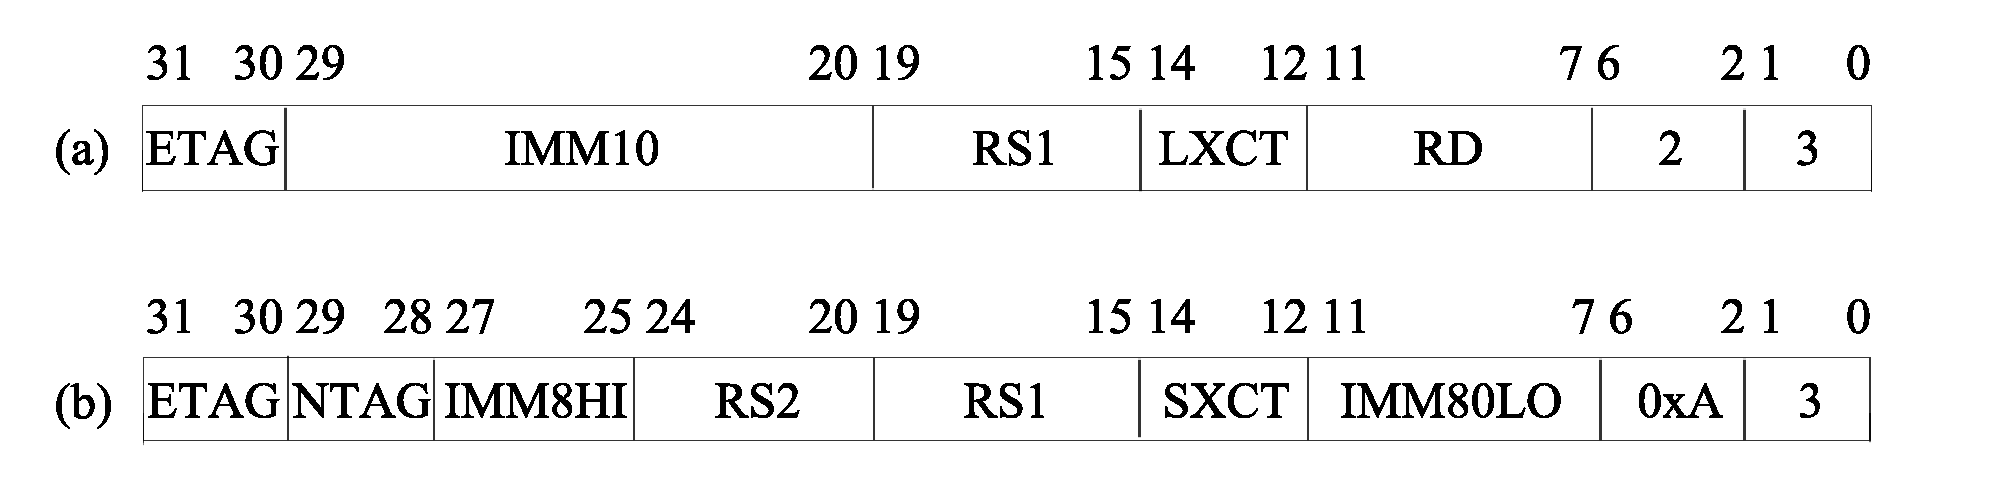
\includegraphics[width=\columnwidth]{asset/LSCT.eps}
	\caption{We extend the original RISC-V instruction architecture with a set of tag-aware instructions to support tagged memory operations. The newly designed instructions are based on I/S type instructions and can perform access control for load and store operations according to the destination memory tag.(a) LCT instructions machine code; (b) SCT instruction machine code.}
	\label{fig:LSCT}
\end{figure}

\subsubsection{Datapath and Decoder Modification}
For the sake of newly designed tag-aware instructions, the CPU also oughts to be modified. In the meanwhile, the decoder is extended to be capable to extract the etag from LCT instructions and the etag and ntag from SCT instructions. Besides, the immediate field is changed so the original signed extension part cannot run correctly. We add a new signed extension module to correctly extract address offset from new instructions just like what has been explained before.

\subsubsection{CPU State Extension}
A branch-new exception state is added to CPU to handle illegal memory operation related with tag policy. When the expected tag in the instruction and the destination memory tag do not match, CPU enters this certain exception state and raises a trap. This exception state makes sure that the tag isolation policy will not be abused, and protects the trusted data from illegal access and modification. It is noteworthy is that upon most occasions malicious attacker could tamper the pointer, like CP or SP, respectively for code text and data segment, which is almost impossible to defend. Hence, what protectors should do is to check whether the pointer is pointing to a correct memory. In this, to protect trusted memory not to be overwritten is the priority action. 

\subsubsection{Tag Policy}
This section will explain the tag policy in SUNFLOWER, including the isolation policy and the update policy. For codes in N-domains, they can read, write data with N-tag and execute code with N-tag, as well as code with TC-tag to enter trusted mode. But codes in N-domains is not allowed to access code or data with TU-tag or TS-tag. For codes in TU-mode, they can read, write data with TU-tag and N-tag. They can execute instructions with TU-tag and TC-tag, and will leave trusted mode when executing codes with N-tag. The codes in TS-mode has access to all the resources. As for the tag update policy, the tags can only be updated under modes with higher or the same security level with itself, i.e. N-tag can be updated in N-domain, TU-mode and TS-mode, while TS-tag can be updated in TU-mode, TS-mode but not in N-domains. Specially, TC-tag can only be updated in TS-mode, to ensure security transform from normal domains to trusted modes. 

% add a table? %

\subsection{Operating System Related Design}

From first RISC-V Proxy Kernel used for beginner's experiments, our project finally determines to use FreeRTOS to build our applications. Based on concept of task, we encapsulate some certain enclave API functions and labels for users, who could simply invoke these achievements without knowing what is working underneath. 

\subsubsection{Basic Execution Environment Theoretical Concept}

Since RISC-V program could not run by itself, applications ,based on RISC-V, need kernel support to work.  For instance, the RISC-V Proxy Kernel, pk, is a lightweight application execution environment that can host statically-linked RISC-V ELF binaries. It is designed to support tethered RISC-V implementations with limited I/O capability and thus handles I/O-related system called by proxying them to a host computer. Tethered System, as its name, refers to those system that cannot stand alone, which means that they may not have complete facilities and depend on a host system to boot. Speaking of boot, pk goes with the Berkly Boot Loader, denoted as bbl. It is the supervisor part of this execution environment and need to handle basic booting work, like initialization.

To be more detailed, RISC-V Proxy Kernel implement a communication between RISC-V Target running proxy kernel and x86 Host running front-end server. The bridge between them is called Host-Target Interface (HTIF), which corresponds to riscv-fesvr project.

At first, many experimentations related our final goal were done by using pk. Then, based on these theoretical concepts learned from pk, our project determines to build applications on FreeRTOS, which is a open source real-time operating system kernel for embedded devices. What is more, it has been ported to RISC-V micro-controller platform. 

\subsubsection{Custom Functions Supported by FreeRTOS Port}

As said before, FreeRTOS could support RISC-V perfectly and detailed implementation is contained in its portable files, to be more specifically, mostly in port.c.  

In this port, it is most significant that we rewrite and complete its syscall trap to support our design. What is noteworthy is that trap in FreeRTOS is generalized trap, which simulates both hardware and software interruption. In this trap, we need to handle a mode-change request, which transfer current mode to machine mode. This design is on the purpose of enclave service management, which need to be dealt with in machine mode. Detailed process is written in assembly language by modifying mstatus register to change current mode.

\subsubsection{Enclave Implementation Details}

Process in FreeRTOS  is called task, which is quite important concept of this operating system. As we all know, in Linux we sometimes call it task, too, like task\_struct. Just like task\_struct, every task in FreeRTOS need a xTaskParameter to initialize, which include information about detailed function to run, its name, stack allocation and so on. Besides this, every task, seen as an individual application, also need another parameter, denoted as xEnclaveRegions, to mark where belongs to enclave, and an function address list, denoted as xTaskEntryPoints, to mark where secure functions begin.

After introducing our resources to be prepared, it is time to figure out our basic idea of enclave implementation. Our aim is to put all memory, which need to be tagged and belongs to these task, together during linking stage. Then if our memory is continuous, it would be much convenient to set tag and do other management. To achieve this purpose, divide memory four part, normal data, normal function, secure data and secure function and denote them using different marks, like NORMAL\_DATA, NORMAL\_FUNCTION, SECURE\_DATA and SECURE\_FUNCTION. These marks correspond to their \_\_attribute\_\_, consist of name, mode, type and position, which could determine a section in memory. Positions are set as ATTR\_MIDDLE firstly and will be explained later.

Position is the most ingenious trick in the method. Create four pointers to mark where normal and secure regions start and end. They have not been initialized, as they are just symbols without any exact meaning now. Then set their positions to ATTR\_START and ATTR\_END. So far, all functions and data are sectioned into chucks of memory.  Hence, in linking stage, pack text and data up, and sort them by using position. In order to do that, we define ATTR\_START as 'a', which is the beginning of alphabet, ATTR\_END as 'z', the ending, and ATTR\_MIDDLE 'b' or other letter in the middle pf 'a' and 'z'. Then the sort could be just implement by linker script using SORT\_BY\_NAME.

Finally, get each part's address at load-time because linker cannot know symbol at link time. In the other words, we do this in task initialization. Until now, we could set enclave and tag uniformly by using our encapsulated API, which would be described in more detailed later.

\subsubsection{Enclave Service API Encapsulation}

Our trusted supervisor provides FreeRTOS a series of API to manipulate enclaves. Every enclave has a structure, denoted as TTCB, to keep information, like region address, magic number for security and so on. In these operating system services, we use mutex lock to maintain mutual exclusiveness of TTCB and tag demanding memory by using checked load and store instructions, which also are encapsulated.

\section{Demo Design}
We design a demo program to show our design works, shown like \ref{fig:demo_code}. Boot loader runs in machine mode, first load our tag service, then is the FreeRTOS kernel. When everything is ready, switch to user mode to run our test program. Part of the memory is allocated for the trusted environment, then TU is marked for this part, and TC is marked for the first instruction as the entry. Then the program and relevant data are loaded, and the trusted program can be called after initialization. When program finished, we will release this part and re-mark the N mark.

\begin{figure}
	\centering{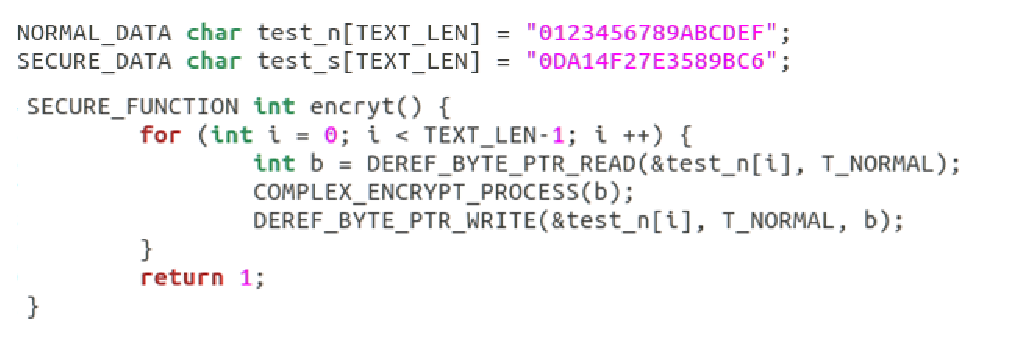
\includegraphics[width=\columnwidth]{asset/Demo2.eps}}
	\caption{The operation of the trust encryption function is to use the tags marked with TU to encrypt the data marked with N, that is to say, use the trust data to encrypt the untrusted data. In the demo, test\_n corresponds to the untrusted data, and test\_s corresponds to the trust data.We encrypt data in bytes. When  trust function is completed, we return to untrusted world and print our encrypted result.}
	\label{fig:demo_code}
\end{figure}

The operation of the trust encryption function is to use the tags marked with TU to encrypt the data marked with N, that is to say, use the trust data to encrypt the untrusted data. In the demo, test\_n corresponds to the untrusted data, and test\_s corresponds to the trust data.We encrypt data in bytes. When  trust function is completed, we return to untrusted world and print our encrypted result, as figure \ref{fig:demo_output} shows.

\begin{figure}
	\centering{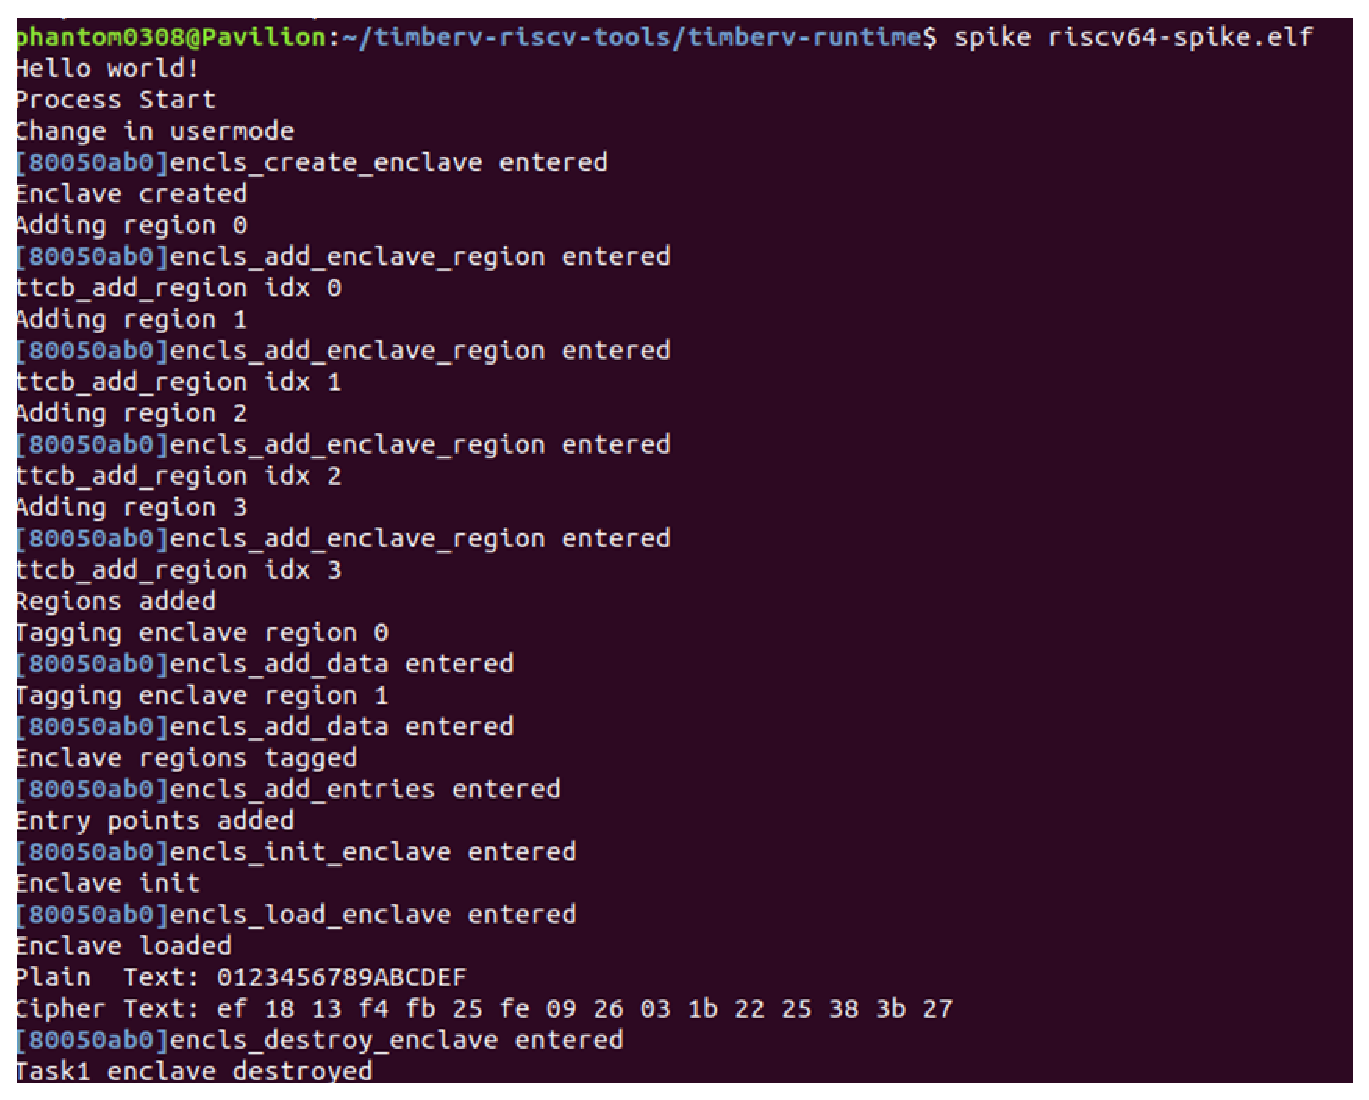
\includegraphics[width=0.7\columnwidth]{asset/Demo4.eps}}
	\caption{Boot loader runs in machine mode, first load our tag service, then is the FreeRTOS kernel. When everything is ready, switch to user mode to run our test program. Part of the memory is allocated for the trusted environment, then TU is marked for this part, and TC is marked for the first instruction as the entry. Then the program and relevant data are loaded, and the trusted program can be called after initialization. When program finished, we will release this part and re-mark the N mark.}
	\label{fig:demo_output}
\end{figure}


At the same time, we designed an untrusted program to try to access the trusted world to prove our design works. As shown in the figure \ref{fig:demo_fail}, this program tried to directly output the key, but it failed, which caused a trap to terminate this process. The following output information is the register content at this time.

\begin{figure}
	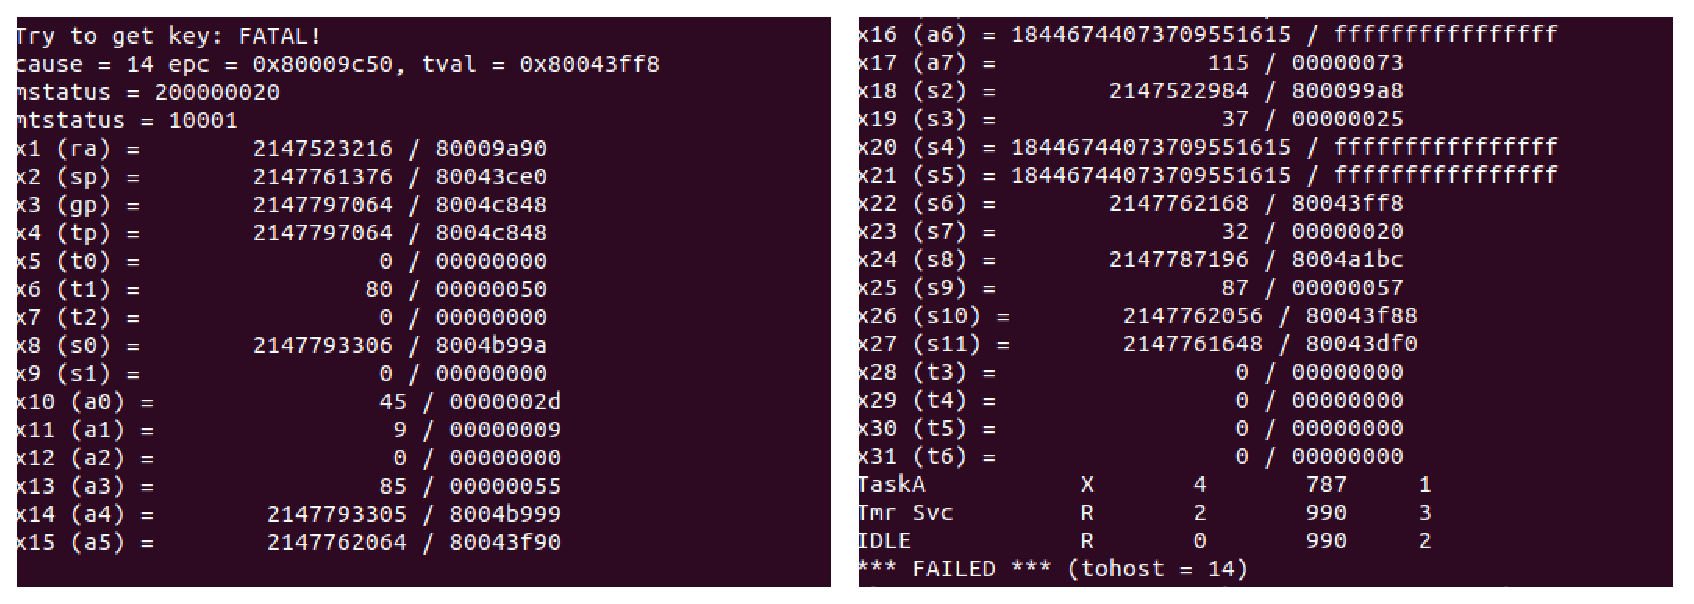
\includegraphics[width=\columnwidth]{asset/Demo1.eps}
	\caption{This program tried to directly output the key, but it failed, which caused a trap to terminate this process. The following output information is the register content at this time.}
	\label{fig:demo_fail}
\end{figure}

% ======================================
% # Future Work and Possible Extension #
% ======================================

\section{Future Work and Possible Extension}
Our project still has many limitations. In one way we have not achieve whole implementation such as MPU part, and in another way we would like to develop more custom applications. 

Without MPU control, it is possible for attacker to crack our trusted zone from other process, since we just check the tag not where they belongs. Hence, In the next few days, our team attempts to add MPU protection. And let MPU set different modes with different privileges, in order to defend outside attack. Based on existing achievements that we have found related port in FreeRTOS, it is not difficult to implement it in certain operating system.

What is more, for our current demo, we did not implement to set tag to lower privileges. But this is a little problem, which will be fixed after appending MPU.

Furthermore, we try to exploit the most development and utilization of our achievements. A typically example is plug-in. Be as specific as possible, plug-ins are supposed not to be able to touch the main application data or function, which owner want to keep secret. Just as demo shows, if a normal function attempts to access secure data, then the task would break down. Beside this kind of specific plug-ins, written in advance during coding, we would like to achieve the case that users could add any custom plug-ins without any secure problems, which is ideal but realizable.


% ==================
% # Conclusion #
% ==================

\section{Conclusion}
This work shows measured results on two X-Band GaN MMIC ($0.15\,\mu m$ process). High efficiencies (higher than $56\%$) are obtained for both amplification and rectification modes. Rectification is performed in self-synchronous way without any injection on the gate RF port. A passive termination is self-sufficient at microwave frequencies thanks to the Miller effect produced by $C_{gd}$ in the HEMT GaN intrinsic non-linear model.


% ==================
% # Acknowledgment #
% ==================

\section*{Acknowledgment}
This work belongs to project of the class, Network Security Theory and Practice, supported by Kai Bu.


% ==============
% # REFERENCES #
% ==============

\begin{thebibliography}{1}

\bibitem{TrustZone} 
\emph{ARM Security Technology: Building a Secure System using TrustZone Technology}, 2009. Ref. no. PRD29-GENC-009492C.

\bibitem{SGX}F. McKeen, I. Alexandrovich, A. Berenzon, C. V. Rozas, H. Shafi, V. Shanbhogue, and U. R. Savagaonkar.
\emph{Innovative instructions and software model for isolated execution. In Hardware and Architectural
Support for Security and Privacy C HASP, ACM, page 10}, 2013. 

\bibitem{TIMBERV}S. Weiser, M. Werner, F. Brasser, M. Malenko, S. Mangard and A. Sadeghi.
\emph{TIMBER-V: Tag-Isolated Memory Bringing Fine-grained Enclaves to RISC-V},
Proc. NDSS, 2019.

\bibitem{HDFI}C. Song, H. Moon, M. Alam, I. Yun, B. Lee, T. Kim, W. Lee, and Y. Paek. 
\emph{HDFI: Hardware-Assisted Data-Flow Isolation},
In Security and Privacy 16, pages 1C17. IEEE Computer Society, 2016.

\bibitem{RISCV}A. Waterman and K. Asanovic. 
\emph{The risc-v instruction set manual,
volume i: User-level isa, version 2.2. Technical report, SiFive Inc},
EECS Department, University of California, Berkeley, 2017.

\end{thebibliography}

\end{document}
